%!TEX root = ../main.tex

\vspace{-0.1em}
\section{Evaluation}
\label{sec:evaluation}

We experimentally evaluate the efficacy of \system{} in three steps.
After describing our setup, we first investigate the efficiency of \system{}.
Next, we analyze our approach's effectiveness.
Lastly, we conduct a set of micro-benchmarks to demonstrate how \system{}'s core parameters jointly influence all dimensions of its performance.

Most importantly, our evaluation shows that \exact{} dominates our baselines in a skyline analysis while \approximate{} is up to more than two orders of magnitude faster than them.

\vspace{-0.3em}
\subsection{Experimental Setup}
\label{sec:setup}

We implemented our prototype for \system{} in Python, leveraging performance optimizations from packages like NumPy and scikit-learn~\cite{pedregosa_scikit-learn_2011}.
Our experiments used an Ubuntu 22.04 server with two Intel Xeon 6330 CPUs (112 vCores @ 2.0GHz) and 512~GB RAM.

\paragraph{Dataset Collections}

\begin{table}[t]
    \caption{Overview of benchmark dataset collections. Size represents the total size of all files in the collection.}
    \label{tab:dataset_collections}
    \centering
    \footnotesize
    \begin{tabularx}{\linewidth}{ >{\raggedright\arraybackslash}X l r r r }
        \toprule
        Name & ID & \# Datasets & Size (GB) & \# Histograms \\
        \midrule
         SportsTables~\cite{langenecker_sportstables_2023}  & ST & $1\;183$      & 0.3 & $19\;862$ \\
         Open Data~\cite{galhotra_metam_2023}               & OD & $5\;966$      & 29  & $68\;313$ \\
         GitTables~\cite{hulsebos_gittables_2023}           & GT & $1\;018\;649$ & 39  & $5\;017\;619$ \\
         \bottomrule
    \end{tabularx}
\end{table}

Table~\ref{tab:dataset_collections} summarizes the three real-world dataset collections we used.
Sports\-Tables~\cite{langenecker_sportstables_2023} is interesting to analyze because it has been explicitly curated to contain many numeric columns with realistic value distributions.
Open Data~\cite{galhotra_metam_2023} is an excerpt of datasets from Open Data Portal Watch~\cite{neumaier_automated_2016}, which aggregates statistics from 280 open data portals, such as NYC Open Data.
Lastly, we used GitTables~\cite{hulsebos_gittables_2023} to evaluate the scalability of \system{}.
None of the collections currently include dataset profiles with histograms, wherefore we downloaded the raw data and generated histograms ourselves.
We randomized the number of bins per histogram to simulate heterogeneous dataset profiles from different data repositories.
The histogram value range and average bin width of Open Data and GitTables span more than 15 orders of magnitude.\looseness=-1

\paragraph{Baselines}
\pscan (Section~\ref{sec:research_challenges}) is a natural baseline for our problem.
We consider the results of \pscan as the ground truth for a query since there is no way to compute a more accurate answer to a percentile predicate based on histograms.
In addition, \binsort is an optimized baseline that precomputes lower and upper percentile estimates for each bin edge and sorts the percentiles by their bin edge.
At query time, \binsort can use binary search on the bin edge domain but has to perform a linear scan over the results to evaluate the percentile requirement since there is no total sort order over both dimensions.
Thus, it represents a middle point between \pscan and \system{}, which is able to leverage binary search on both dimensions.
To evaluate the space-efficiency of \system{}, we furthermore introduce \ndist, which approximates each numerical column with a normal distribution and thus only has to store two values per column instead of $\cB_c$ values per histogram.
Note that while \ndist is space-efficient, it does not achieve a sublinear execution time, as the two parameters of a normal distribution do not have a total ordering in one dimension.

\paragraph{Benchmark Queries}
To the best of our knowledge, there is no benchmark for dis\-tri\-bu\-tion-aware dataset search queries, requiring us to define the set of evaluation queries ourselves.
Since there also is no widely agreed-upon metric to estimate the ``difficulty'' of a dataset search query in terms of answering it quickly and accurately, we randomly generated a diverse set of $10\;000$ queries with percentile predicates and categorized them based on three different metrics:
query selectivity describes the percentage of histograms a query matches (e.g.,~0.9 means that 90\% of the histograms match a query);
the share of cluster matches measures the number of clusters in an index that a predicate's value range overlaps with (since \system{} can directly tell if all or no histograms in a cluster match a predicate if the value ranges do not overlap);
finally, the bin edge matches count how many original histogram bin edges fall on the edge of a predicate's value range (because predicates with many matches might be harder to evaluate accurately after aligning the histogram bins).
In a preliminary experiment, we analyzed the value distribution of each metric across the generated queries and our dataset collections.
We observed that the query selectivity metric splits the queries into subsets with a high (>90\%), medium (10-90\%), or low (<10\%) selectivity, whereas the other two metrics did not prove to be robust query categorizations.
Most predicate ranges overlap with 10-40\% of the clusters, while the number of exact matches with the original bin edges is zero for next to all queries.
Therefore, we categorized based on query selectivity and randomly sampled 333 queries from each selectivity group to collate a diverse set of 999 benchmark queries.
In addition, we sampled another 100 queries per category to obtain a set of 300 queries that we used for a comprehensive grid search (see Section~\ref{sec:solution_effectiveness}) to identify the best parameters of our index.\looseness=-1


\subsection{Solution Efficiency}
\label{sec:solution_efficiency}

We start our evaluation of \system{} with an efficiency analysis and present five experiments: a runtime comparison, a scalability analysis, runtime breakdowns of \approximate{} and \textsc{Exact}, and an index construction time analysis.
Since \ndist has no runtime advantage over \pscan, we omit it in this section.

\paragraph{Runtime Comparison}

\begin{figure}[t]
    \centering
    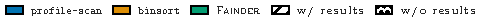
\includegraphics{figures/figure_10_legend.pdf}\\
    \begin{subfigure}[t]{.03\linewidth}
        \centering
        
\includegraphics{figures/figure_10_label.pdf}
    \end{subfigure}%
    \hspace{-0.005\linewidth}%
    \begin{subfigure}[t]{.325\linewidth}
        \centering
        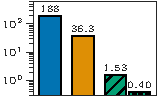
\includegraphics{figures/figure_10_a.pdf}
        \caption{SportsTables}
    \end{subfigure}%
    \begin{subfigure}[t]{.325\linewidth}
        \centering
        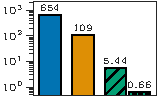
\includegraphics{figures/figure_10_b.pdf}
        \caption{Open Data}
    \end{subfigure}%
    \begin{subfigure}[t]{.325\linewidth}
        \centering
        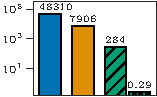
\includegraphics{figures/figure_10_c.pdf}
        \caption{GitTables}
    \end{subfigure}%
    \caption{Runtime comparison of \pscan, \binsort, and \approximate{} over 999 queries.}
    \Description{Bar chart showing runtime across all solutions and datasets.}
    \label{fig:runtime_comparison}
    % Figure width: 78.3722pt / 1.08in / 27mm
\end{figure}

\begin{figure}[t]
    \centering
    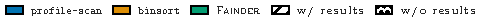
\includegraphics{figures/figure_11_legend.pdf}\\
    \begin{subfigure}[t]{.03\linewidth}
        \centering
        
\includegraphics{figures/figure_11_label.pdf}
    \end{subfigure}%
    \hspace{-0.005\linewidth}%
    \begin{subfigure}[t]{.325\linewidth}
        \centering
        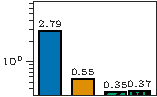
\includegraphics{figures/figure_11_a.pdf}
        \caption{SportsTables}
    \end{subfigure}%
    \begin{subfigure}[t]{.325\linewidth}
        \centering
        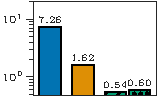
\includegraphics{figures/figure_11_b.pdf}
        \caption{Open Data}
    \end{subfigure}%
    \begin{subfigure}[t]{.325\linewidth}
        \centering
        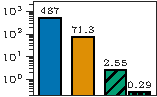
\includegraphics{figures/figure_11_c.pdf}
        \caption{GitTables}
    \end{subfigure}%
    \caption{Runtime comparison of \pscan, \binsort, and \approximate{} over 999 queries with low selectivity.}
    \Description{Bar chart showing runtime for low selectivity queries across all solutions and datasets.}
    \label{fig:runtime_comparison_low_selectivity}
    % Figure width: 78.3722pt / 1.08in / 27mm
\end{figure}

Figure~\ref{fig:runtime_comparison} shows an execution time comparison for our 999 test queries.
The figure highlights that \approximate{} is more than two orders of magnitude faster than \pscan and $20-28\times$ faster than \binsort on all three dataset collections.
Furthermore, we observe that \approximate{} achieves interactive execution times for each collection if we scale down the runtime to an individual predicate evaluation.

As we only benchmark the runtime of individual percentile predicates instead of large composite queries in this experiment, the result set $S$ can become quite large.
Therefore, we also ran a modified version of \system{} that performs all steps from Algorithm~\ref{alg:index_query} until line~\ref{alg:after_cluster} but returns a dummy result of size 1 to filter out the linear time impact of processing the result set.
This ``without results'' execution time demonstrates the potential runtime impact of $S$.
While the difference to the regular execution of \system{} is $4-5\times$ for SportsTables and Open Data, \system{} is another two orders of magnitude faster on GitTables when not returning results.
This shows how significant \system{}'s runtime advantage over the baselines is if the execution is not dominated by $S$ -- either because users run composite queries with multiple different predicates or because a percentile predicate itself has very low selectivity.

To specifically test the runtime of \system{} when a percentile predicate has very low selectivity, we simulated a restrictive column identifier that only matches 1\% of the histograms and then ran our benchmark queries on the resulting histogram subset.
The average selectivity of our queries when combining the column identifier and the distributional requirement lies at 0.5\%.
Figure~\ref{fig:runtime_comparison_low_selectivity} highlights that \system{} maintains its performance lead over the baselines for low-selectivity queries, while the relative advantage shrinks for the small dataset collections SportsTables and Open Data.
This is because \system{}'s runtime grows or shrinks logarithmically with the collection size while the baselines benefit linearly from a smaller collection.
We also see that the result set $S$ no longer impacts the runtime for the small collections.
Regarding GitTables, about $10\;000$ histograms remain after prefiltering so that \system{} still outperforms all baselines by orders of magnitude, consistent with Figure~\ref{fig:runtime_comparison}.
Overall, the experiment shows that \system{} is a superior choice in terms of runtime, especially for large-scale dataset search.

\paragraph{Scalability}
We investigate the scalability of \system{} by creating four versions of our largest collection GitTables, including each histogram 0.25, 0.5, 1, and 2 times on average to achieve a respective scaling factor.
Figure~\ref{fig:runtime_scalability} summarizes the runtime of \system{} for all scaling factors.
To account for the impact of the solution size $S$, we again conduct the experiment with and without processing the search results.
We see that the execution time of the runs that return results increases linearly with the scaling factor since $|S|$ also increases linearly with the scaling factor.
Contrarily, the runtime of \system{} is almost constant without returning results, highlighting its logarithmic scaling in the number of histograms and bins.

\paragraph{\approximate{}}

\begin{figure}[t]
    \centering
    \begin{minipage}[b]{0.47\linewidth}
        \centering
        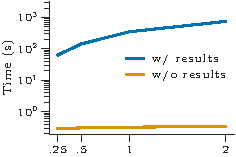
\includegraphics{figures/figure_12.pdf}
        \caption{Runtime on Git\-Tables across scaling factors.}
        \Description{Line chart showing runtime over scaling factor.}
        \label{fig:runtime_scalability}
        % Figure width: 113.33961pt / 1.568in / 39.8mm
    \end{minipage}%
    \hfill%
    \begin{minipage}[b]{0.49\linewidth}
        \centering
        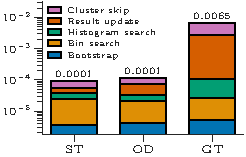
\includegraphics{figures/figure_13.pdf}
        \caption{Predicate evaluation runtime breakdown.}
        \Description{Stacked bar chart showing runtime of each \system{} phase over each dataset collection.}
        \label{fig:runtime_breakdown}
        % Figure width: 118.16359pt / 1.635in / 41.5mm
    \end{minipage}
\end{figure}

After reviewing the scalability of \system{}, we zoom into the individual phases of predicate evaluation with \approximate{}.
Due to the challenges of tracing a system-under-test without altering its performance~\cite{jain_art_1991}, we only measure the conceptually necessary steps of \system{} in this experiment.
Note that tracing those steps already increases a query's execution time by one order of magnitude due to logging overhead.

Figure~\ref{fig:runtime_breakdown} dissects the core operations of our index for the exemplary predicate $\cP_{*, 0.1, <, 50}$.
The experiment shows that the two most critical operations, bin and histogram search, scale sublinearly with the dataset collection size.
While bin search time is almost the same across collections, histogram search only grows by $7\times$ for GitTables, although the collection is $252\times$ and $73\times$ larger than the other two collections.
The result set update, on the other hand, scales linearly with $|S|$ and thus takes noticeably more time for GitTables.
Cluster skip partially also scales with $|S|$ as all histograms from a cluster might have to be added to $S$ depending on line~\ref{alg:cluster_skip} in Algorithm~\ref{alg:index_query}.

\paragraph{\exact{}}

\begin{figure}[t]
    \centering
    
\includegraphics{figures/figure_14_legend.pdf}\\
    \begin{subfigure}[t]{.03\linewidth}
        \centering
        
\includegraphics{figures/figure_14_label.pdf}
    \end{subfigure}%
    \hspace{-0.005\linewidth}%
    \begin{subfigure}[t]{.325\linewidth}
        \centering
        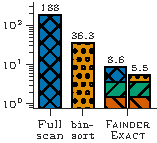
\includegraphics{figures/figure_14_a.pdf}
        \caption{SportsTables}
    \end{subfigure}%
    \begin{subfigure}[t]{.325\linewidth}
        \centering
        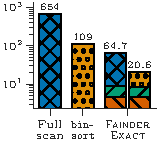
\includegraphics{figures/figure_14_b.pdf}
        \caption{Open Data}
    \end{subfigure}%
    \begin{subfigure}[t]{.325\linewidth}
        \centering
        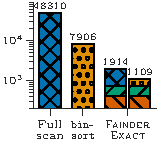
\includegraphics{figures/figure_14_c.pdf}
        \caption{GitTables}
    \end{subfigure}%
    \caption{Execution time breakdown of \exact{} compared to baselines for 999 queries.}
    \Description{Four bar charts showing the runtime of \pscan, \binsort, and \exact{} for each dataset collection.}
    \label{fig:exact_results}
\end{figure}

Building on the analysis of \approximate{}, we investigate the efficiency of our exact solution.
Figure~\ref{fig:exact_results} shows the runtime of its three phases compared to our exact baselines.
Since \pscan and \binsort both yield exact results, we can use either for the third stage of \exact{}.
Conceptually, \exact{} has no guaranteed speedup as the improvement depends on the combined pruning factor of the first two stages.
Nevertheless, in practice, it is $10-25\times$ faster than \pscan and $5-7\times$ faster than \binsort, as it can prune (a)~98\%, (b)~93\%, and (c)~98\% of the histograms on average for our benchmark queries.
Noticeably, the third iterative stage still dominates the runtime in many cases.\looseness=-1

Note that while \binsort appears like an overall better baseline, its performance depends not only on the number of histograms in a collection but also on the number of bins per histogram, as it creates an index entry for each bin.
However, we cannot control the number of bins per histogram in our setting since they are created by the data owners.
In a side experiment, we verified that the runtime of \binsort increases linearly if we simulate collections with more average bins per histogram.
Therefore, the optimal algorithm choice for stage three depends on the histogram collection, while both choices generally yield speedups over the baselines.

\paragraph{Index Construction}

\begin{figure}[t]
    \centering
    
\includegraphics{figures/figure_15_legend.pdf}\\
    \begin{subfigure}[t]{.03\linewidth}
        \centering
        
\includegraphics{figures/figure_15_label.pdf}
    \end{subfigure}%
    % \hspace{-0.6em}
    \begin{subfigure}[t]{.485\linewidth}
        \centering
        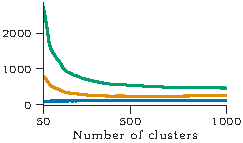
\includegraphics{figures/figure_15_a.pdf}
    \end{subfigure}%
    \begin{subfigure}[t]{.485\linewidth}
        \centering
        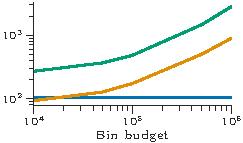
\includegraphics{figures/figure_15_b.pdf}
    \end{subfigure}%
    \caption{Construction time of \system{} on GitTables with a bin budget of $\boldsymbol{50\;000}$ (left) and 100 clusters (right).}
    \Description{Two line charts showing the runtime over the number of clusters (left) and the bin budget (right).}
    \label{fig:construction_time_gittables}
    % Figure width: 116.95668pt / 1.61in / 41.1mm
\end{figure}

In Figure~\ref{fig:construction_time_gittables}, we measure the index construction time on GitTables and vary the number of clusters $k$ while keeping the bin budget $\cB$ fixed and vice versa.
We divide index construction time into clustering and histogram alignment, separating rebinning and conversion for histogram alignment.
We observe that the impact of $k$ and $\cB$ on clustering time is negligible, as k-Means has robust scalability and \system{}'s aligned bins are only assigned after the histograms have been clustered.
Rebinning and conversion time decreases with an increasing $k$ because the index becomes smaller with more evenly distributed clusters, resulting in fewer percentiles to compute.
Conversely, $\cB$ increases histogram alignment time by increasing the number of percentiles in the index.
Overall, the index construction time for a reasonable selection of $k$ is feasible, considering that histogram insertion and deletion are incremental.
We only need to construct \system{} from scratch at the beginning or when processing significant bulk updates.


\subsection{Solution Effectiveness}
\label{sec:solution_effectiveness}

We analyze the effectiveness of \system{} in three parts:
We discuss a qualitative case study of distribution-aware dataset search on existing search engines, examine the findings of our hyperparameter grid search, and finally compare \system{}'s accuracy with our baselines.\looseness=-1

\paragraph{Case Study}
We conducted a qualitative case study to estimate the time a human needs to run a search with percentile requirements, combining keyword queries and manual investigation.
For this, we continued our initial motivating example to show the current user experience's shortcomings concretely.
We used Kaggle Datasets~\cite{kaggle_inc_kaggle_2024} in our study, as it is a comprehensive collection of datasets specifically intended for machine learning (i.e.,~a use case that benefits from percentile predicates).
As of February 2024, our example's keyword query ``lung cancer age'' yielded 67 results that our data scientist needs to review.
We make a conservative estimate and assume they need one minute per dataset on average, including datasets they can quickly rule out and datasets they have to download and analyze with a tool like Pandas.
This would take them about one hour instead of less than a second with \system{}.
Since users often search for datasets in a work context, this showcases the considerable economic potential of distribution-aware search.

\begin{figure*}[t]
    \setlength{\belowcaptionskip}{-4mm}
    \centering
    
\includegraphics{figures/figure_16_legend.pdf}\\
    \begin{subfigure}[t]{.03\linewidth}
        \centering
        
\includegraphics{figures/figure_16_label.pdf}
    \end{subfigure}%
    \hspace{-0.005\linewidth}%
    \begin{subfigure}[t]{.325\linewidth}
        \centering
        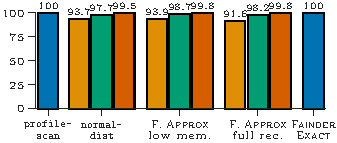
\includegraphics{figures/figure_16_a.pdf}
        \caption{SportsTables}
    \end{subfigure}%
    \begin{subfigure}[t]{.325\linewidth}
        \centering
        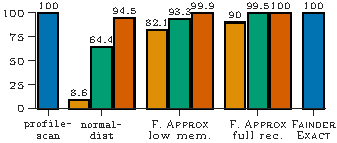
\includegraphics{figures/figure_16_b.pdf}
        \caption{Open Data}
    \end{subfigure}%
    \begin{subfigure}[t]{.325\linewidth}
        \centering
        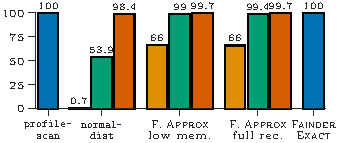
\includegraphics{figures/figure_16_c.pdf}
        \caption{GitTables}
    \end{subfigure}%
    \caption{$\boldsymbol{F_1}$ score of \pscan, \ndist, \approximate{}, and \exact{}, grouped by query selectivity.}
    \Description{Bar chart showing the $F_1$ score of each solution grouped by query selectivity and dataset collection.}
    \label{fig:accuracy_barchart_f1}
    % Figure width: 164.54433pt / 2.27in / 57.8mm
\end{figure*}

\paragraph{Hyperparameter Grid Search}
We conducted an extensive grid search on our validation query set to analyze \system{}'s configuration robustness.
Below, we summarize our key insights regarding the choice of clustering algorithm ($A$), clustering feature transformation ($T$), number of clusters ($k$), and bin budget ($\cB$).

($A$)
We examined three classes of clustering algorithms: density-based clustering with HDBSCAN~\cite{campello_density-based_2013}, agglomerative clustering, and k-Means.
Density-based clustering does not require choosing the hyperparameter $k$.
However, it can classify an arbitrarily large share of points as outliers.
This is detrimental in our setting since we need to index all histograms, and forming a heterogeneous outlier cluster yields catastrophic query accuracy within that cluster.
Agglomerative clustering makes no assumptions about the feature distribution and is robust to outliers.
Yet, it does not achieve a feasible runtime for large dataset collections; we aborted a grid search on GitTables because it took more than 2.5 days, while k-Means took less than 5 hours for the same search.
k-Means achieved the best overall performance, producing clusterings that yield accurate indices within less than two minutes for each dataset collection.

($T$)
Next to a quantile transform~\cite{pedregosa_scikit-learn_2011}, we also investigated simple and robust standardization, as well as no feature preprocessing in our experiments.
If the features fall into clearly separable clusters by default, such as with SportsTables, we found that simple standardization or no preprocessing can yield the best results.
However, across dataset collections and index configurations, the quantile transform is most robust to heterogeneous histogram features and thus produces the smallest and most accurate indices on average.

($k$)
Using a reasonably large value for $k$ (> 100) generally yields a good result accuracy.
Increasing $k$ beyond this point presents a trade-off between index size and runtime, as $k$ has a linear impact on the runtime but reduces the number of computed percentiles.

($\cB$)
The bin budget should be chosen according to the memory capacity and in conjunction with $k$, as more clusters result in smaller indices.
A higher bin budget generally produces more precise indices, although with diminishing returns.

Based on our grid search results, we selected index configurations that optimize result accuracy and reduce the index size for our other experiments.
Concretely, we use k-Means and preprocess all collections but SportsTables using a quantile transform.
In addition, we use (230, 250, 750) clusters and (5K, 50K, 100K) bins for SportsTables, Open Data, and GitTables.

\paragraph{Accuracy Comparison}
Figure~\ref{fig:accuracy_barchart_f1} presents the $F_1$ score of \pscan, \ndist, \approximate{} low memory (based on rebinning), \approximate{} full recall (based on conversion), as well as \exact{}.
For the approximate solutions, we group the results by query selectivity.
We observe that all approaches perform best on SportsTables, with its manually curated datasets that often match a normal distribution.
For Open Data and GitTables, the results are more diverse.
\ndist performs consistently worse than \approximate{} variants, especially on the more challenging collections.
\approximate{} constructed with conversion performs better than rebinning on Open Data due to its guaranteed recall of 1 but at the cost of using more memory.
Overall, low and medium selectivity queries have a lower $F_1$ score.

\begin{figure}[t]
    \setlength{\belowcaptionskip}{-1mm}
    \centering
    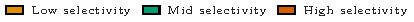
\includegraphics{figures/figure_17_legend.pdf}\\
    \begin{subfigure}[t]{.49\linewidth}
        \centering
        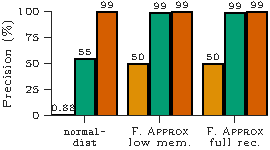
\includegraphics[scale=0.91]{figures/figure_17_a.pdf}
    \end{subfigure}%
    \hfill%
    \begin{subfigure}[t]{.49\linewidth}
        \centering
        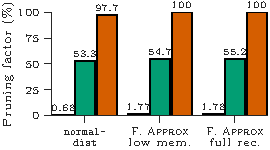
\includegraphics[scale=0.91]{figures/figure_17_b.pdf}
    \end{subfigure}%
    \caption{Precision and pruning factor of approximate solutions on GitTables.}
    \Description{Two bar charts showing the precision (left) and pruning factor (right) of the approximate solutions on GitTables, grouped by query selectivity.}
    \label{fig:accuracy_barchart_approx}
    % Figure width: 118.16359pt / 1.63in / 41.5mm
\end{figure}

To explain the worse $F_1$ score for queries with lower selectivity, we show the precision and pruning factor of approximate solutions on GitTables in Figure~\ref{fig:accuracy_barchart_approx}.
Comparing the results to the $F_1$ score from Figure~\ref{fig:accuracy_barchart_f1}~(c), we observe that a lower precision predominantly causes the performance decrease.
Considering the pruning factor, we see that \approximate{} variants nevertheless filter out around 98\% of the histograms.
If the cardinality of the true result is low, a small absolute number of false positives can cause a sizeable relative performance decrease in precision.
Thus, we argue that the worse performance for low selectivity queries has limited practical impact, as the absolute number of false results is small.

\begin{figure}[t]
    \setlength{\belowcaptionskip}{-2mm}
    \centering
    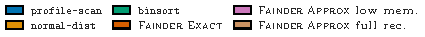
\includegraphics{figures/figure_18_legend.pdf}\\
    \begin{subfigure}[t]{.03\linewidth}
        \centering
        
\includegraphics{figures/figure_18_label.pdf}
    \end{subfigure}%
    \hspace{-0.005\linewidth}%
    \begin{subfigure}[t]{.325\linewidth}
        \centering
        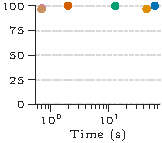
\includegraphics{figures/figure_18_a.pdf}
        \caption{SportsTables}
    \end{subfigure}%
    \begin{subfigure}[t]{.325\linewidth}
        \centering
        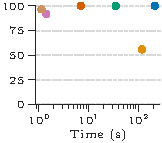
\includegraphics{figures/figure_18_b.pdf}
        \caption{Open Data}
    \end{subfigure}%
    \begin{subfigure}[t]{.325\linewidth}
        \centering
        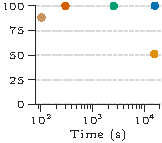
\includegraphics{figures/figure_18_c.pdf}
        \caption{GitTables}
    \end{subfigure}%
    \caption{$\boldsymbol{F_1}$ score over runtime of \pscan, \ndist, \binsort, and \system{} variants.}
    \Description{Three scatter plots showing the $F_1$ score over the runtime of all solutions across the three dataset collections.}
    \label{fig:accuracy_scatterplot_f1}
\end{figure}

We also jointly investigated each approach's result accuracy and runtime performance.
Figure~\ref{fig:accuracy_scatterplot_f1} highlights that \system{} strictly dominates the baselines in a skyline analysis for all three dataset collections.
\exact{} achieves 100\% $F_1$ score in $5-53\times$ less time than the exact baselines.
\approximate{} variants achieve the fastest runtime overall at the cost of producing a few false results.
\ndist presents a worse accuracy-runtime trade-off than our solutions on all collections.
Therefore, we argue that its space savings ($O(2)$ vs. $O(\cB_c)$ per column) are not justified unless the vast majority of columns follow a normal distribution.


\subsection{Micro-Benchmarks}
\label{sec:micro_benchmarks}

We conclude our experimental evaluation with a holistic analysis of the impact of the number of clusters and the bin budget on all three dimensions of \system{}'s performance.
Finally, we distill our investigation into two easy-to-follow steps for practitioners.

\paragraph{Impact of Clustering}

\begin{figure}[t]
    \centering
    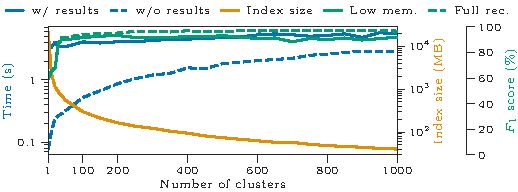
\includegraphics[scale=0.965]{figures/figure_19.pdf}
    \caption{Query runtime, index size, and $\boldsymbol{F_1}$ score of \approximate{} over the number of clusters on Open Data.}
    \Description{Line chart with three y-axes showing the runtime, index size, and $F_1$ score of \system{} over the number of clusters on Open Data.}
    \label{fig:microbenchmark_open_data_k}
    % Figure width: 241.14749pt / 3.33in / 84.7mm
\end{figure}

Figure~\ref{fig:microbenchmark_open_data_k} demonstrates the interplay of runtime, result accuracy, and index size for a varying number of clusters and $50\;000$ bins on Open Data.
Without a sufficient number of clusters ($k<10$ in this case), accuracy and index size deteriorate significantly as the aligned bins become less precise and the clusters less balanced.
For $k=1$, the memory consumption (and index construction time) becomes unfeasible.
Thus, clustering is a critical component of \system{}.
Fortunately, the choice of $k$ for larger values is robust concerning the result accuracy, making \system{} easy to configure.
This experiment supports our grid search's finding that increasing $k$ presents a trade-off between index size and runtime.
However, when comparing the two blue lines, we see that the runtime impact of a growing $k$ is partly mitigated if we also consider the result processing time.
This is because more clusters can yield a more precise index, resulting in a smaller result set size.\looseness=-1


\paragraph{Impact of Bin Budget}

\begin{figure}[t]
    \centering
    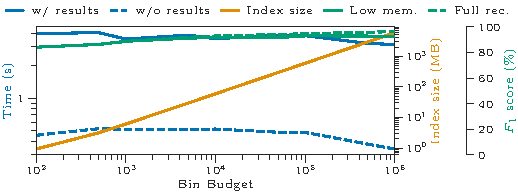
\includegraphics[scale=0.965]{figures/figure_20.pdf}
    \caption{Query runtime, index size, and $\boldsymbol{F_1}$ score of \approximate{} over varying bin budgets on Open Data.}
    \Description{Line chart with three y-axes showing the runtime, index size, and $F_1$ score of \system{} over the bin budget on Open Data.}
    \label{fig:microbenchmark_open_data_b}
\end{figure}

In Figure~\ref{fig:microbenchmark_open_data_b}, we fix the number of clusters to 100 and vary the bin budget.
We observe that (1) the runtime is robust to the bin budget due to our use of binary search; (2) the $F_1$ score increases from 84\% to 93\% and 96\% with an increasing bin budget, although at diminishing returns; and (3) the index size grows linearly with $\cB$.
Note that, in general, the size of \system{} scales with the number but not the size of the datasets.
This makes \system{} relatively large for dataset collections with many small datasets, such as GitTables.
On the other side, it is robust to dataset collections for machine learning, where individual datasets can take up many gigabytes or even terabytes of storage.

\paragraph{Practical Guidance for Index Configuration}
First, select the largest possible value of $k$ acceptable for runtime.
To ensure performance, $k$ should be at least $100\times$ smaller than $|\cH|$.
Then, choose the largest possible value of $\cB$ acceptable in terms of index size.
